\documentclass[tikz,border=8pt]{standalone}
\usepackage{tikz}
\usepackage{pgfplots}
\usepackage{amsmath,amssymb}
\usepackage[T1]{fontenc}
\usepackage{lmodern}
\usepackage{xcolor}
\usetikzlibrary{arrows.meta,positioning,shapes.geometric,fit,calc,backgrounds,matrix}
\pgfplotsset{compat=1.18}
\definecolor{ink}{HTML}{18202A}
\definecolor{blue}{HTML}{2563EB}
\definecolor{bluefill}{HTML}{EAF1FF}
\definecolor{green}{HTML}{14804A}
\definecolor{greenfill}{HTML}{E8F6EE}
\definecolor{amber}{HTML}{B56A00}
\definecolor{amberfill}{HTML}{FFF3D6}
\definecolor{red}{HTML}{B42318}
\definecolor{redfill}{HTML}{FDECEC}
\definecolor{gray}{HTML}{667085}
\definecolor{light}{HTML}{F4F6F8}
\definecolor{linegray}{HTML}{C7CDD4}
\tikzset{
  box/.style={draw=ink, rounded corners=3pt, very thick, fill=white, align=center, inner sep=7pt, font=\sffamily\small},
  bluebox/.style={box, fill=bluefill, draw=blue},
  greenbox/.style={box, fill=greenfill, draw=green},
  amberbox/.style={box, fill=amberfill, draw=amber},
  redbox/.style={box, fill=redfill, draw=red},
  ghost/.style={draw=linegray, rounded corners=3pt, thick, fill=light, align=center, inner sep=7pt, font=\sffamily\small},
  label/.style={font=\sffamily\footnotesize, text=gray, align=center},
  title/.style={font=\sffamily\bfseries\large, text=ink, align=center},
  arrow/.style={-{Latex[length=3mm,width=2mm]}, very thick, draw=ink},
  bluearrow/.style={-{Latex[length=3mm,width=2mm]}, very thick, draw=blue},
  redarrow/.style={-{Latex[length=3mm,width=2mm]}, very thick, draw=red},
  greenarrow/.style={-{Latex[length=3mm,width=2mm]}, very thick, draw=green}
}

\begin{document}
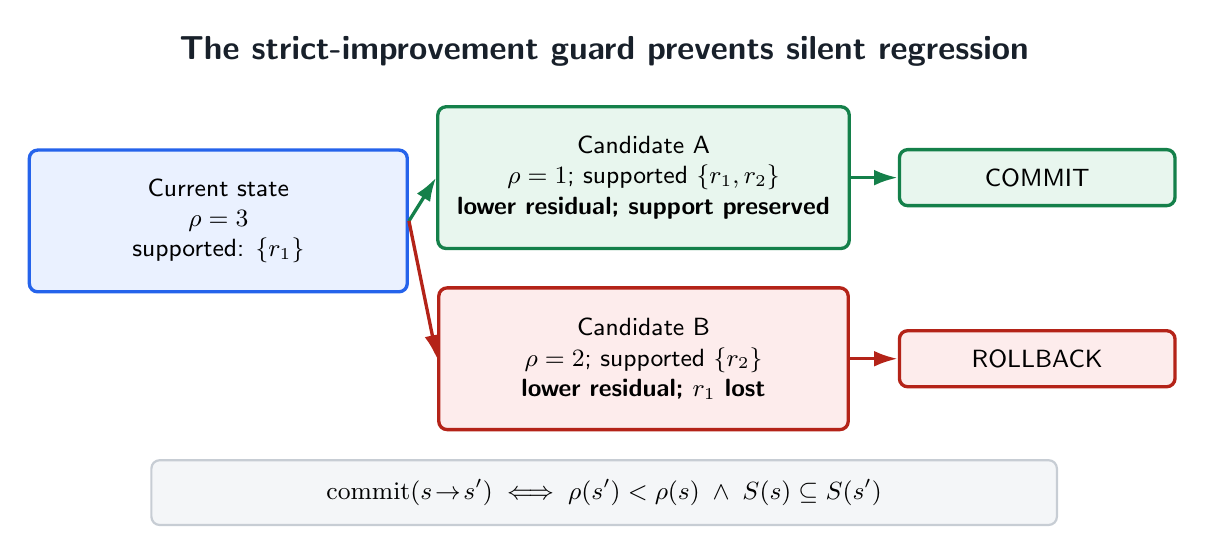
\begin{tikzpicture}
\node[title] at (7.5,4.85) {The strict-improvement guard prevents silent regression};
\node[bluebox, minimum width=48mm, minimum height=18mm] (old) at (2.6,2.7) {Current state\\$\rho=3$\\supported: $\{r_1\}$};
\node[greenbox, minimum width=52mm, minimum height=18mm] (good) at (8.0,3.25) {Candidate A\\$\rho=1$; supported $\{r_1,r_2\}$\\\textbf{lower residual; support preserved}};
\node[redbox, minimum width=52mm, minimum height=18mm] (bad) at (8.0,0.95) {Candidate B\\$\rho=2$; supported $\{r_2\}$\\\textbf{lower residual; $r_1$ lost}};
\draw[greenarrow] (old.east)--(good.west);
\draw[redarrow] (old.east)--(bad.west);
\node[greenbox, minimum width=35mm] (c) at (13.0,3.25) {COMMIT};
\node[redbox, minimum width=35mm] (r) at (13.0,0.95) {ROLLBACK};
\draw[greenarrow] (good.east)--(c.west); \draw[redarrow] (bad.east)--(r.west);
\node[ghost, minimum width=115mm] at (7.5,-0.75) {$\mathrm{commit}(s\!\to\!s') \iff \rho(s')<\rho(s)\;\land\;S(s)\subseteq S(s')$};
\end{tikzpicture}
\end{document}
